\documentclass[10pt, letterpaper, twocolumn]{article}

% --- Packages ---
\usepackage[utf8]{inputenc}
\usepackage[left=0.5in, right=0.5in, top=0.5in, bottom=0.75in, columnsep=0.25in]{geometry}
\usepackage{amsmath, amssymb, amsfonts}
\usepackage{cite}
\usepackage{hyperref}
\usepackage{booktabs}
\usepackage[runin]{abstract}
\usepackage{changepage}
\usepackage{graphicx}
\usepackage{placeins}
\usepackage{listings}
\usepackage{xcolor}

% --- Formatting Abstract ---
\renewcommand{\abstractnamefont}{\normalfont\bfseries}
\renewcommand{\abstracttextfont}{\normalfont\small}
\abslabeldelim{- }

% --- Listings style for inline code blocks ---
\lstset{
    basicstyle=\ttfamily\footnotesize,
    breaklines=true,
    columns=fullflexible,
    frame=single,
    framesep=3pt,
    xleftmargin=2pt,
    xrightmargin=2pt,
    keepspaces=true,
    showstringspaces=false
}

% --- Metadata ---
\title{\Large \bfseries [Project Report] Adding AF\_XDP I/O Backend Support to mTCP: A User-level TCP Stack for Multicore Systems}
\author{
    {\Large Toshit Jain} \\
    {\large Roll No: 230101106} \\
    {\large \texttt{j.toshit@iitg.ac.in}}
}
\date{}

\begin{document}

\maketitle

\begin{abstract}
\noindent This report documents the design, implementation, and testing of an AF\_XDP I/O backend for the mTCP user-level TCP stack. mTCP originally relied on kernel-bypass frameworks such as DPDK, netmap, PSIO, and ONVM, all of which require either proprietary userspace drivers, NIC unbinding, or specialised hardware. The objective of this work was to make mTCP run on stock Linux kernels (5.x and above) by introducing a new I/O module built on top of AF\_XDP sockets, an in-kernel eBPF-XDP program, and a shared UMEM-backed packet buffer pool. The resulting backend preserves mTCP's per-core, batch-oriented architecture while removing the requirement of unbinding NICs from the kernel. The implementation was developed and validated end-to-end on CloudLab bare-metal nodes.
\end{abstract}

\section{What is eBPF, AF\_XDP and how do they work?}

\textit{This section is the study that I did before starting the implementation. I had no prior exposure to in-kernel programmable packet pipelines, so I documented the building blocks here for completeness.}

\subsection{eBPF (Extended Berkeley Packet Filter)}

eBPF is an in-kernel virtual machine that allows safe, sandboxed bytecode programs to be attached to well-defined hook points inside the Linux kernel without modifying or recompiling the kernel itself. eBPF programs are written in a restricted C dialect, compiled to eBPF bytecode by Clang/LLVM, verified by the kernel verifier (which proves bounded loops, valid memory accesses, and termination), and then JIT-compiled to native instructions. They communicate with userspace through \texttt{bpf} maps, which are kernel-resident key-value containers of fixed type and size, accessible from both the program and userspace via the \texttt{bpf()} syscall.

\subsection{XDP (eXpress Data Path)}

XDP is the earliest hook point in the Linux receive path. An XDP program runs on every packet \textit{before} a \texttt{sk\_buff} is allocated, which makes it dramatically cheaper than tc-bpf or netfilter-based filtering. The program inspects the raw frame and returns one of four verdicts:
\begin{itemize}
    \item \texttt{XDP\_PASS} -- forward the packet up the regular Linux stack as if XDP were absent.
    \item \texttt{XDP\_DROP} -- discard the packet immediately, without any further processing.
    \item \texttt{XDP\_TX} -- bounce the packet back out the same NIC.
    \item \texttt{XDP\_REDIRECT} -- send the packet to another destination such as a different NIC, a CPU, or, most importantly for this project, an AF\_XDP socket.
\end{itemize}
XDP can run in three modes: \texttt{generic} (SKB mode, after \texttt{sk\_buff} allocation), \texttt{native} (driver-level, the default fast path), and \texttt{offloaded} (executed on capable NIC hardware).

\subsection{AF\_XDP}

AF\_XDP is a Linux socket family introduced in kernel 4.18 and matured through the 5.x series. It exposes a userspace ring-buffer interface that exchanges raw frames with the kernel at near-DPDK speeds, but with two crucial differences: it does not require a userspace NIC driver, and it does not require the NIC to be unbound from the kernel. The NIC remains under normal kernel control, which means that traffic that the userspace application does not claim continues to be served by the kernel's networking stack as usual.

An AF\_XDP socket (commonly called an \texttt{xsk}) is bound to a specific (NIC, RX queue) pair. When an XDP program returns \texttt{XDP\_REDIRECT} into a special map of type \texttt{BPF\_MAP\_TYPE\_XSKMAP}, the frame is dropped directly into that socket's userspace ring instead of continuing through the kernel.

\subsection{UMEM and the Four Rings}

The data plane of every AF\_XDP socket revolves around two abstractions:

\begin{itemize}
    \item \textbf{UMEM:} A contiguous region of userspace memory, registered with the kernel, that backs every ring. The kernel writes incoming packets into UMEM frames; userspace reads them in place (\textit{zero-copy}). Outgoing packets are also constructed inside UMEM frames before being handed to the kernel.
    \item \textbf{Four rings per socket:}
    \begin{itemize}
        \item \texttt{RX} -- kernel produces, userspace consumes (received frames).
        \item \texttt{TX} -- userspace produces, kernel consumes (frames to send).
        \item \texttt{FQ} (Fill Queue) -- userspace gives the kernel free UMEM frames for the kernel to write incoming packets into.
        \item \texttt{CQ} (Completion Queue) -- kernel returns UMEM frames to userspace once their TX has completed, so that userspace can recycle them.
    \end{itemize}
\end{itemize}

% --- Optional figure placeholder for AF_XDP architecture ---
\begin{figure}[htbp]
    \centering
    % \includegraphics[width=0.48\textwidth]{afxdp_overview.png}
    \fbox{\parbox[c][1.7in][c]{0.45\textwidth}{\centering\textit{[SS placeholder: high-level AF\_XDP architecture\\(NIC $\to$ XDP $\to$ XSKMAP $\to$ UMEM rings $\to$ userspace)]}}}
    \caption{High-level data flow of AF\_XDP. Place screenshot/diagram here.}
    \label{fig:afxdp_overview}
\end{figure}
\FloatBarrier

\subsection{Why this combination matters for mTCP}

mTCP's original design assumes a fast, batched, userspace packet I/O abstraction. DPDK satisfies this but at the cost of removing the NIC from the kernel and requiring hugepages and a userspace driver. AF\_XDP gives mTCP a similar batched, ring-based packet pipeline while keeping the NIC under kernel ownership: traffic that mTCP doesn't want (e.g. SSH on the management interface) can be sent back to the kernel via \texttt{XDP\_PASS}, eliminating the operational pain of dual-port test setups. This is the central reason for adding AF\_XDP as a first-class I/O backend.

\section{Brief description of current I/O modules}

mTCP is intentionally pluggable at the packet I/O layer. A common interface, \texttt{struct io\_module\_func}, declares a fixed set of callbacks (\texttt{load\_module}, \texttt{init\_handle}, \texttt{link\_devices}, \texttt{recv\_pkts}, \texttt{get\_rptr}, \texttt{send\_pkts}, \texttt{get\_wptr}, \texttt{release\_pkt}, \texttt{select}, \texttt{destroy\_handle}, \texttt{dev\_ioctl}). Each backend implements this interface in a dedicated translation unit. Before the AF\_XDP work, the upstream tree shipped four backends.

\subsection{PSIO (\texttt{psio\_module.c})}

PSIO is the original packet I/O layer that the NSDI'14 paper used for its measurements. It is built on the Packet Shader I/O Engine and requires a custom kernel module plus a patched Intel \texttt{ixgbe} driver. PSIO exposes batched RX/TX rings to userspace and was the primary reason mTCP could match line-rate on 10\,GbE in the original paper. Its main downside today is portability: the kernel patches are tied to specific kernel and driver versions and have not been actively maintained for modern kernels.

\subsection{DPDK (\texttt{dpdk\_module.c})}

DPDK is the most commonly used backend in current deployments. It uses Poll Mode Drivers (PMDs) running entirely in userspace, hugepages for memory allocation, and a fully unbound NIC. The mTCP DPDK module translates the \texttt{io\_module\_func} calls into \texttt{rte\_eth\_*} operations, with one TX/RX queue per mTCP thread. DPDK gives the highest absolute throughput but demands hugepage configuration, exclusive ownership of the NIC, and either VFIO or UIO bindings -- all of which complicate operation on shared or remotely managed test machines.

\subsection{netmap (\texttt{netmap\_module.c})}

netmap is a kernel-resident framework that exposes preallocated NIC rings directly to userspace via \texttt{mmap}. It does not require unbinding the NIC entirely, but does require a netmap-aware driver. It is lighter weight than DPDK but considerably less ubiquitous, and on most modern Linux distributions an explicit out-of-tree build is necessary.

\subsection{ONVM (\texttt{onvm\_module.c})}

ONVM (Open Network Function Manager) layers a Network Function (NF) abstraction on top of DPDK. Multiple NFs share a single DPDK port, with the ONVM manager dispatching packets between them via service IDs. The ONVM mTCP module is therefore conceptually a thin wrapper that hands packets to the ONVM runtime rather than to a NIC directly. It inherits all DPDK setup overhead.

\subsection{Why a fifth (AF\_XDP) backend was added}

All four existing backends require either out-of-tree drivers, kernel patches, exclusive NIC ownership, or hugepage setup. None of them work on a stock Linux 5.x machine where the NIC must remain available for SSH and management traffic. AF\_XDP closes exactly this gap. The new \texttt{afxdp\_module.c} implements the same \texttt{io\_module\_func} interface, but routes traffic through an in-kernel XDP/eBPF program (\texttt{afxdp\_kern.c}) and AF\_XDP sockets, with no driver patching and no NIC unbinding.

\begin{figure}[htbp]
    \centering
    % \includegraphics[width=0.48\textwidth]{io_module_layout.png}
    \fbox{\parbox[c][1.4in][c]{0.45\textwidth}{\centering\textit{[SS placeholder: block diagram of mTCP\\with five pluggable I/O modules\\selected via \texttt{io = afxdp} in config]}}}
    \caption{The mTCP I/O module abstraction with the new AF\_XDP backend. Place diagram here.}
    \label{fig:io_modules}
\end{figure}
\FloatBarrier

\section{Description of \texttt{afxdp\_kern.c}}

\texttt{afxdp\_kern.c} is the in-kernel half of the new backend. It is compiled as an eBPF object file (\texttt{afxdp\_kern.o}) by Clang in \texttt{-target bpf -O2 -g} mode, attached to each NIC that mTCP claims, and verified by the kernel before execution. Its sole job is to decide, on a per-packet basis, whether a frame should be redirected into an mTCP-owned AF\_XDP socket or allowed to continue up the regular Linux stack.

\subsection{Includes and the \texttt{xsks\_map}}

The file is a CO-RE / BTF-based program: it includes \texttt{vmlinux.h} (generated once via \texttt{bpftool btf dump file /sys/kernel/btf/vmlinux format c}), so all kernel types resolve at verification time without depending on installed kernel headers. It then declares the central data structure -- the redirect map:

\begin{lstlisting}[language=C]
struct {
    __uint(type, BPF_MAP_TYPE_XSKMAP);
    __uint(max_entries, 256);
    __uint(key_size,   sizeof(__u32));
    __uint(value_size, sizeof(__u32));
} xsks_map SEC(".maps");
\end{lstlisting}

This is a map of type \texttt{BPF\_MAP\_TYPE\_XSKMAP}, the dedicated map type for AF\_XDP redirects. The userspace half (\texttt{afxdp\_module.c}) populates an entry in this map for every AF\_XDP socket it creates; the kernel program looks up an entry and uses \texttt{bpf\_redirect\_map} to deliver the packet into that socket.

\subsection{The \texttt{xdp\_sock\_prog} entry function}

The single program in this file is \texttt{xdp\_sock\_prog}, tagged with \texttt{SEC("xdp")}. It receives an \texttt{xdp\_md} context from the kernel, from which it extracts \texttt{data} and \texttt{data\_end} pointers. The function logic proceeds in three stages:

\begin{itemize}
    \item \textbf{Header bounds check:} Before reading any field, the program checks that the next header is fully within the packet (\texttt{(void *)(eth + 1) > data\_end}). The eBPF verifier requires these checks; without them the program will be rejected at load time. The same pattern is applied for the IPv4 and TCP headers.
    \item \textbf{SSH carve-out:} If the packet is IPv4/TCP and the source or destination port is 22, the program returns \texttt{XDP\_PASS} unconditionally. This is critical for remote testbeds (such as CloudLab) where the only access path to the node is SSH on the same NIC. Without this carve-out, the very first \texttt{xdp\_program\_\_attach} call would lock the operator out of the machine.
    \item \textbf{Default redirect to AF\_XDP:} For every other packet, the program reads \texttt{ctx->rx\_queue\_index}, looks it up in \texttt{xsks\_map}, and -- if present -- calls \texttt{bpf\_redirect\_map(\&xsks\_map, index, XDP\_PASS)}. The third argument specifies the fallback action if the map entry is missing, so misconfigured queues never silently drop traffic. A \texttt{BPF\_PRINTK} call writes a one-line trace to \texttt{/sys/kernel/debug/tracing/trace\_pipe} for every redirect decision; this proved invaluable during debugging.
\end{itemize}

\begin{figure}[htbp]
    \centering
    % 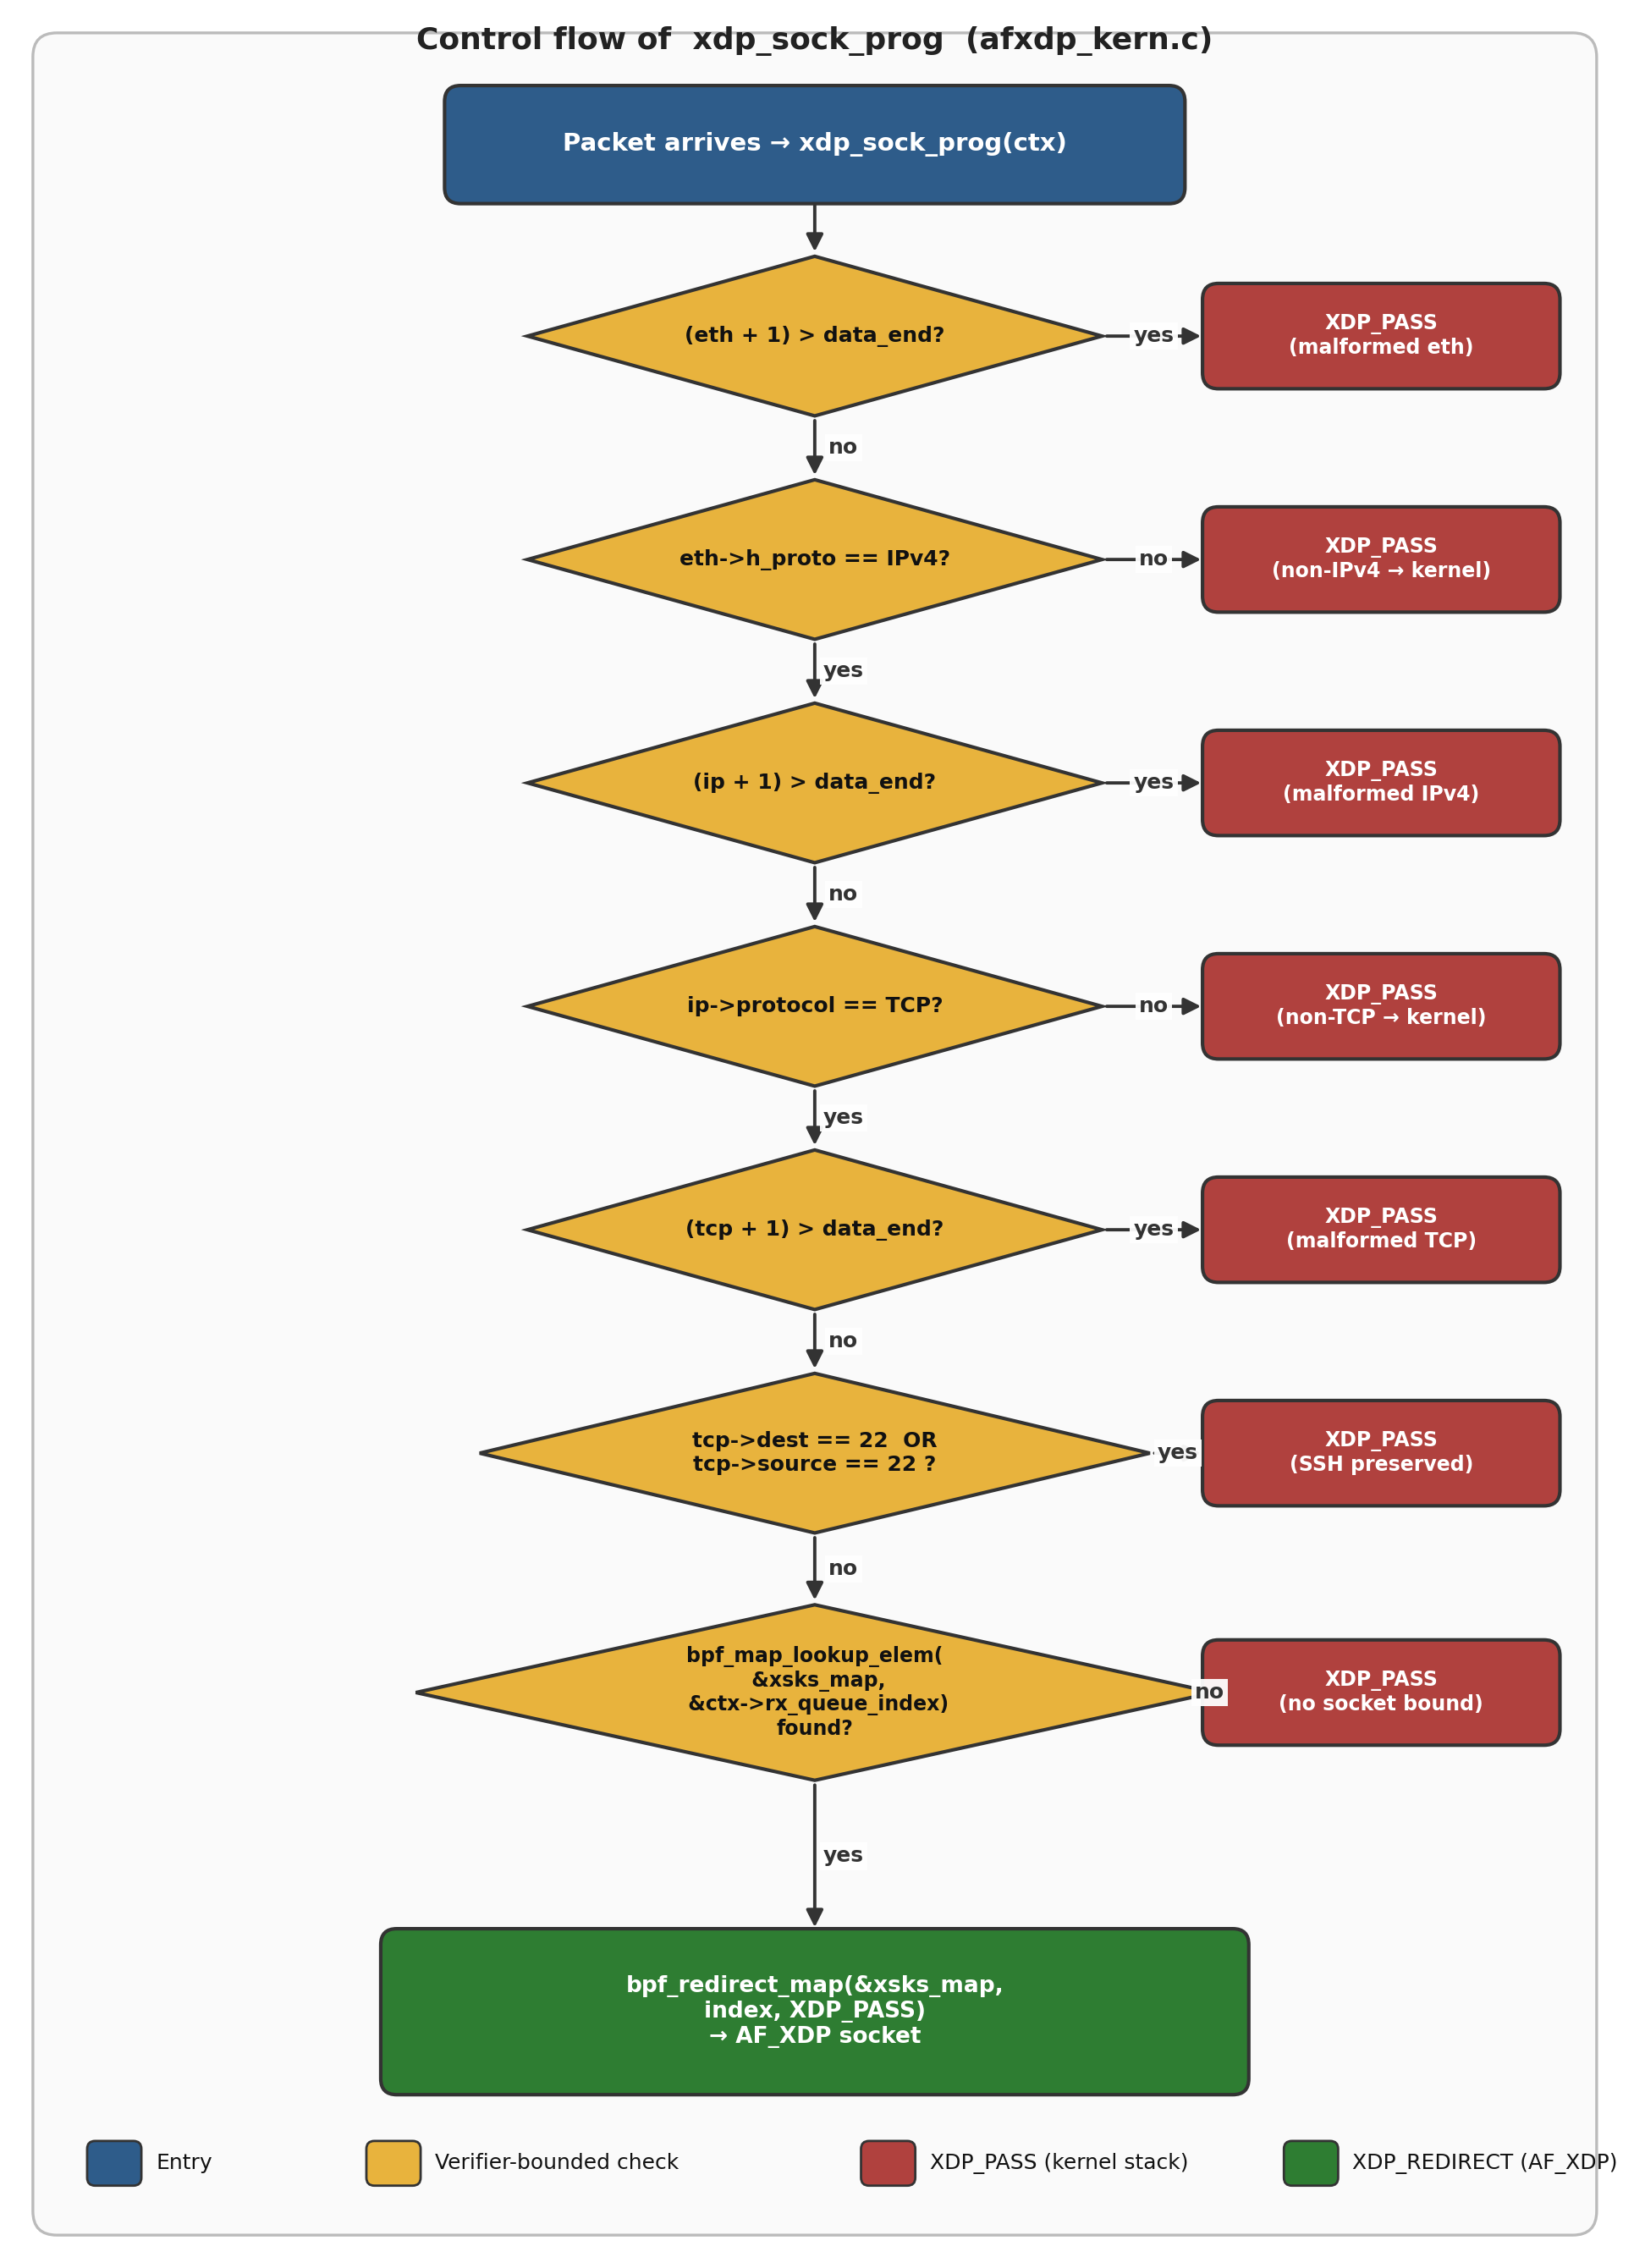
\includegraphics[width=0.48\textwidth]{kern_decision_tree.png}
    \fbox{\parbox[c][1.7in][c]{0.45\textwidth}{\centering\textit{[SS placeholder: control-flow of\\\texttt{xdp\_sock\_prog}: bounds checks\\$\to$ SSH carve-out $\to$ redirect map]}}}
    \caption{Control flow of \texttt{xdp\_sock\_prog} inside \texttt{afxdp\_kern.c}. Place screenshot here.}
    \label{fig:kern_flow}
\end{figure}
\FloatBarrier

\subsection{Frame-key mapping caveat}

The current implementation keys \texttt{xsks\_map} by \texttt{ctx->rx\_queue\_index}. This is sufficient for the intended single-data-interface, single-queue setup. However, in a multi-NIC topology where each NIC has only queue 0, every socket would land at \texttt{xsks\_map[0]} and overwrite each other (last write wins). The fix, documented in the kern file's header comment, is to switch to composite keying using \texttt{(ctx->ingress\_ifindex, ctx->rx\_queue\_index)} on the kernel side, with matching \texttt{bpf\_map\_update\_elem(\dots,\&kernel\_ifindex,\dots)} on the userspace side.

\subsection{Licensing and build}

The license is set to \texttt{GPL} via the \texttt{\_license} \texttt{SEC} entry. This is mandatory because several BPF helpers (including \texttt{bpf\_trace\_printk}) are GPL-only. The Makefile rule responsible for the object file is:
\begin{lstlisting}[language=bash]
afxdp_kern.o: afxdp_kern.c
    $(BPF_CLANG) $(BPF_CFLAGS) -c $< -o $@
\end{lstlisting}
where \texttt{BPF\_CLANG} defaults to \texttt{clang} and \texttt{BPF\_CFLAGS} to \texttt{-target bpf -O2 -g}. The resulting \texttt{afxdp\_kern.o} is loaded at runtime by the userspace half via \texttt{xdp\_program\_\_create}.

\section{Description of \texttt{afxdp\_module.c} (function-wise)}

\texttt{afxdp\_module.c} is the userspace half of the backend. It implements every callback in \texttt{io\_module\_func} on top of \texttt{libxdp}'s AF\_XDP socket API. The file is wrapped in \texttt{\#ifndef DISABLE\_AFXDP \dots \#else \dots \#endif} so that the compilation unit collapses to a stub when \texttt{--enable-afxdp} is not passed to \texttt{configure}.

\subsection{Compile-time configuration and core data structures}

The module pins a small number of compile-time constants:
\begin{itemize}
    \item \texttt{NUM\_FRAMES = 16384} -- total UMEM frames per mTCP thread.
    \item \texttt{FRAME\_SIZE = XSK\_UMEM\_\_DEFAULT\_FRAME\_SIZE} -- frame size, taken straight from libxdp.
    \item \texttt{RX\_BATCH\_SIZE = TX\_BATCH\_SIZE = 64}.
    \item \texttt{RX\_RING\_SIZE = 1024}, \texttt{TX\_RING\_SIZE = 512}.
    \item \texttt{FQ\_RING\_SIZE = 4096} (deliberately large to avoid RX starvation), \texttt{CQ\_RING\_SIZE = 2048}.
\end{itemize}
Two structures back the runtime state:
\begin{itemize}
    \item \texttt{struct xsk\_umem\_info} -- the UMEM, its FQ, its CQ, and the backing buffer pointer. There is exactly one of these per mTCP thread.
    \item \texttt{struct xsk\_socket\_info} -- per-thread state: the UMEM, an array of \texttt{xsk\_if\_socket} (one per attached interface), the free-frame stack, the outstanding TX counter, and per-interface RX/TX batch staging arrays. The struct is 64-byte aligned to avoid false sharing between threads.
\end{itemize}

\subsection{\texttt{afxdp\_load\_module}}

This function runs once globally during \texttt{mtcp\_init()}. Its responsibilities, in order, are:
\begin{itemize}
    \item Resolve the path to \texttt{afxdp\_kern.o}. The path is read from the \texttt{AFXDP\_KERN\_PATH} environment variable, falling back to a Makefile-provided default.
    \item Set \texttt{LIBXDP\_SKIP\_DISPATCHER=1} so that libxdp does not try to install its multi-program dispatcher (mTCP only needs the single XDP program).
    \item Call \texttt{xdp\_program\_\_create()} on \texttt{afxdp\_kern.o}, then \texttt{bpf\_object\_\_load()}. Any verifier rejection is reported with a hint about \texttt{AFXDP\_KERN\_PATH}.
    \item Iterate over \texttt{devices\_attached[]} (populated by \texttt{io\_module.c}) and call \texttt{xdp\_program\_\_attach(\dots, XDP\_MODE\_NATIVE, 0)} for each interface. The chosen attach mode is recorded in \texttt{attached\_mode[ifidx]} so that cleanup can detach with the same mode.
    \item Enable promiscuous mode on every attached interface via \texttt{SIOCSIFFLAGS}; without this, the NIC would drop frames not destined to its own MAC.
    \item Resolve the \texttt{xsks\_map} fd by name (\texttt{bpf\_object\_\_find\_map\_by\_name(obj, "xsks\_map")}) and cache it as a static module variable. Every per-thread socket inserts its fd into this map.
    \item Register \texttt{afxdp\_prog\_cleanup} via \texttt{atexit()} so that the XDP program is detached even on abnormal exit.
\end{itemize}

\begin{figure}[htbp]
    \centering
    % \includegraphics[width=0.48\textwidth]{load_module_screenshot.png}
    \fbox{\parbox[c][1.6in][c]{0.45\textwidth}{\centering\textit{[SS placeholder: \texttt{afxdp\_load\_module}\\source listing or runtime log\\``\texttt{AFXDP: attached XDP \dots}'']}}}
    \caption{\texttt{afxdp\_load\_module} attaches the BPF object on every claimed interface. Place screenshot here.}
    \label{fig:load_module}
\end{figure}
\FloatBarrier

\subsection{\texttt{afxdp\_init\_handle}}

This callback runs once \textit{per mTCP thread} (i.e. per core). The thread-local state is built top-down:
\begin{itemize}
    \item \texttt{setrlimit(RLIMIT\_MEMLOCK, RLIM\_INFINITY)}. UMEM is locked into RAM, so the default 64\,KB memlock cap will fail at \texttt{xsk\_umem\_\_create} time.
    \item Allocate \texttt{NUM\_FRAMES * FRAME\_SIZE} bytes of page-aligned memory via \texttt{posix\_memalign} and pass it to \texttt{configure\_xsk\_umem()}, which calls \texttt{xsk\_umem\_\_create} with the configured FQ/CQ/frame sizes.
    \item Stash the resulting \texttt{xsk\_socket\_info} on \texttt{ctxt->io\_private\_context}; mTCP hands this pointer back to every subsequent callback.
    \item Initialise the free-frame stack (\texttt{umem\_frame\_addr[i] = i*FRAME\_SIZE}) and pre-fill the FQ with \texttt{FQ\_RING\_SIZE} (4096) frames so that the kernel has somewhere to write incoming packets immediately after socket creation.
    \item For every entry in \texttt{CONFIG.eths[]} that has a non-empty \texttt{dev\_name}, call \texttt{xsk\_configure\_socket()} with \texttt{queue\_id = ctxt->cpu}. The first socket on the thread uses \texttt{xsk\_socket\_\_create} (which owns the UMEM); every subsequent socket uses \texttt{xsk\_socket\_\_create\_shared}, sharing the FQ/CQ/UMEM with its sibling sockets on the same core.
\end{itemize}

\subsection{\texttt{xsk\_configure\_socket} (helper)}

Builds an \texttt{xsk\_socket\_config} with \texttt{XDP\_USE\_NEED\_WAKEUP} (so the kernel can be optionally woken up via \texttt{sendto}/\texttt{recvfrom} system calls when its driver thread is asleep) and \texttt{XSK\_LIBBPF\_FLAGS\_\_INHIBIT\_PROG\_LOAD} (so libxdp does not try to load its own default XDP program -- ours is already attached). After the socket is created, the function inserts the AF\_XDP socket fd into \texttt{xsks\_map[queue\_id]} via \texttt{bpf\_map\_update\_elem}.

\subsection{\texttt{configure\_xsk\_umem} / \texttt{xsk\_alloc\_umem\_frame} / \texttt{xsk\_free\_umem\_frame} (helpers)}

\texttt{configure\_xsk\_umem} wraps \texttt{xsk\_umem\_\_create} with the chosen FQ/CQ ring sizes. The other two are tiny stack helpers over \texttt{umem\_frame\_addr[]}: \texttt{alloc} pops a frame for either FQ pre-fill or TX, \texttt{free} pushes a frame back when an RX descriptor has been recycled or a TX completion has been reaped. \texttt{INVALID\_UMEM\_FRAME = UINT64\_MAX} is the sentinel for ``out of frames''.

\subsection{\texttt{afxdp\_get\_wptr}}

Called by mTCP every time it needs to construct an outgoing packet. The function:
\begin{itemize}
    \item Bails if the per-interface TX batch is already full (\texttt{cnt >= TX\_BATCH\_SIZE}).
    \item Allocates one UMEM frame via \texttt{xsk\_alloc\_umem\_frame}.
    \item Stores the frame address and \texttt{len} into the per-interface staging slot \texttt{tx\_batch[ifidx]}, then returns \texttt{xsk\_umem\_\_get\_data(buffer, addr)} so mTCP can write the packet directly into the UMEM frame (true zero-copy on TX).
\end{itemize}

\subsection{\texttt{afxdp\_send\_pkts} and \texttt{complete\_tx} (helper)}

\texttt{complete\_tx} reaps the CQ via \texttt{xsk\_ring\_cons\_\_peek}, returns each completed descriptor's frame to the free stack, and decrements \texttt{outstanding\_tx}. \texttt{afxdp\_send\_pkts} then:
\begin{itemize}
    \item Calls \texttt{complete\_tx} first, so freed frames can immediately be reused.
    \item Reserves \texttt{cnt} slots on the TX ring with \texttt{xsk\_ring\_prod\_\_reserve}; if the reservation is short, the function returns 0 (mTCP will retry).
    \item Fills each \texttt{xdp\_desc} with \texttt{(addr, len)} from the staged batch, then calls \texttt{xsk\_ring\_prod\_\_submit}.
    \item If the kernel needs a wake-up (\texttt{xsk\_ring\_prod\_\_needs\_wakeup}), issues a \texttt{sendto(\dots, MSG\_DONTWAIT, \dots)} kick.
    \item Resets \texttt{tx\_batch[nif].cnt} to zero so the next batch can begin staging.
\end{itemize}

\begin{figure}[htbp]
    \centering
    % \includegraphics[width=0.48\textwidth]{send_pkts_screenshot.png}
    \fbox{\parbox[c][1.6in][c]{0.45\textwidth}{\centering\textit{[SS placeholder: source of\\\texttt{afxdp\_send\_pkts} +\\\texttt{complete\_tx} side-by-side]}}}
    \caption{TX path: \texttt{afxdp\_get\_wptr} stages, \texttt{afxdp\_send\_pkts} submits, \texttt{complete\_tx} reaps. Place screenshot here.}
    \label{fig:send_path}
\end{figure}
\FloatBarrier

\subsection{\texttt{afxdp\_recv\_pkts} and \texttt{afxdp\_get\_rptr}}

The RX path mirrors the TX path:
\begin{itemize}
    \item \texttt{afxdp\_recv\_pkts} first recycles the previous RX batch back into the FQ. For each address staged in \texttt{rx\_batch[ifidx]}, it pushes the address back into the FQ via \texttt{xsk\_ring\_prod\_\_fill\_addr}, then submits.
    \item If the FQ needs a wake-up, it issues a \texttt{recvfrom(\dots, MSG\_DONTWAIT, \dots)} kick.
    \item It then calls \texttt{xsk\_ring\_cons\_\_peek} on the RX ring with \texttt{RX\_BATCH\_SIZE = 64} as the upper bound. Each returned descriptor's \texttt{(addr, len)} is recorded into \texttt{rx\_batch[ifidx]} and the RX ring is released.
    \item \texttt{afxdp\_get\_rptr} is the random-access counterpart for mTCP's per-packet processing loop. Given an interface and an index into the most recent RX batch, it returns the userspace pointer (\texttt{xsk\_umem\_\_get\_data}) and length for that frame. mTCP processes the packet in place; the frame address remains in \texttt{rx\_batch} until the next \texttt{afxdp\_recv\_pkts} call recycles it.
\end{itemize}

\subsection{\texttt{afxdp\_release\_pkt}, \texttt{afxdp\_link\_devices}, \texttt{afxdp\_select}}

These are stubs in the AF\_XDP backend. \texttt{afxdp\_release\_pkt} is a no-op because frame reclamation already happens implicitly inside \texttt{afxdp\_recv\_pkts}. \texttt{afxdp\_link\_devices} returns 0 because the actual link work is done up front in \texttt{afxdp\_load\_module}. \texttt{afxdp\_select} is a placeholder for a future RX-idleness optimisation.

\subsection{\texttt{afxdp\_dev\_ioctl}}

Returns \texttt{-1} unconditionally. The consequence is that mTCP falls back to its software checksum implementation on both RX (verification) and TX (generation). This is a deliberate trade-off; see Section~7.

\subsection{\texttt{afxdp\_destroy\_handle} and \texttt{afxdp\_prog\_cleanup}}

The two functions are intentionally separate. \texttt{afxdp\_destroy\_handle} runs once per thread and frees thread-local state (\texttt{xsk\_socket\_\_delete} for every per-interface socket, \texttt{xsk\_umem\_\_delete}, free of the buffer, free of the \texttt{xsk\_socket\_info} itself). \texttt{afxdp\_prog\_cleanup} is registered globally with \texttt{atexit}, runs exactly once, and detaches the XDP program from every interface using the mode recorded in \texttt{attached\_mode[ifidx]}. Splitting these two responsibilities was necessary because doing the detach inside \texttt{destroy\_handle} caused a race when multiple threads tried to detach the same program from the same interface concurrently.

\subsection{The \texttt{io\_module\_func} vtable}

At the bottom of the file:
\begin{lstlisting}[language=C]
struct io_module_func afxdp_module_func = {
    .load_module    = afxdp_load_module,
    .init_handle    = afxdp_init_handle,
    .link_devices   = afxdp_link_devices,
    .release_pkt    = afxdp_release_pkt,
    .send_pkts      = afxdp_send_pkts,
    .get_wptr       = afxdp_get_wptr,
    .recv_pkts      = afxdp_recv_pkts,
    .get_rptr       = afxdp_get_rptr,
    .select         = afxdp_select,
    .destroy_handle = afxdp_destroy_handle,
    .dev_ioctl      = afxdp_dev_ioctl,
};
\end{lstlisting}
This vtable is what \texttt{io\_module.c} eventually selects when a configuration file specifies \texttt{io = afxdp}.

\section{Testing on CloudLab}

CloudLab \cite{cloudlab} provides free, time-bounded access to bare-metal servers for academic research. It was the only practical environment available to me with full root access, programmable NICs, and the ability to load arbitrary kernel modules and BPF programs. All testing of the AF\_XDP backend was carried out on CloudLab nodes.

\subsection{Logging in and setting up the nodes}

The standard workflow is:
\begin{itemize}
    \item Log in to \href{https://cloudlab.us}{cloudlab.us} with an institutional identity.
    \item Instantiate an experiment from a profile that provides bare-metal Ubuntu 22.04 nodes (the \texttt{small-lan} profile is sufficient: two nodes connected by an experiment-only link).
    \item Wait for the experiment to enter the \texttt{ready} state. The portal then exposes per-node SSH endpoints. The management interface is the one that resolves the SSH endpoint; the experiment interface is the second NIC, typically named \texttt{eno1d1} (or similar) and visible only on the internal experiment LAN.
    \item SSH into both nodes from a local terminal. The first node is designated as the \textit{server} (where mTCP and \texttt{epserver} run); the second as the \textit{client} (where \texttt{curl} runs against the server).
\end{itemize}

\begin{figure}[htbp]
    \centering
    % \includegraphics[width=0.48\textwidth]{cloudlab_topology.png}
    \fbox{\parbox[c][1.6in][c]{0.45\textwidth}{\centering\textit{[SS placeholder: CloudLab\\experiment topology view -- two nodes,\\management iface + experiment iface]}}}
    \caption{CloudLab two-node experiment topology. Place screenshot here.}
    \label{fig:cloudlab_topo}
\end{figure}
\FloatBarrier

\subsection{Setting up environment and RSS using bash scripts}

The repository ships a single \texttt{setup\_linux\_afxdp\_env.sh} script that handles the entire environment bring-up. It is meant to be run as a regular user (it escalates with \texttt{sudo} where required) and is idempotent, so re-running it is safe. Concretely it performs:
\begin{itemize}
    \item \texttt{apt update} and installation of build essentials: \texttt{build-essential}, \texttt{git}, \texttt{clang}, \texttt{llvm}, \texttt{gcc}, \texttt{make}, \texttt{pkg-config}.
    \item Installation of \texttt{linux-tools-\$(uname -r)} so that \texttt{bpftool} is available, plus a symlink into \texttt{/usr/local/sbin}.
    \item Installation of headers and dev libraries: \texttt{libelf-dev}, \texttt{zlib1g-dev}, \texttt{libnuma-dev}, \texttt{libpcap-dev}, \texttt{libgmp-dev}, \texttt{libbpf-dev}, plus \texttt{m4} and \texttt{autoconf}.
    \item Cloning and building \texttt{xdp-project/xdp-tools} (which provides \texttt{libxdp}). Distro packages for \texttt{libxdp-dev} were not available on Ubuntu 22.04 at the time of development, hence the source build.
    \item Adding \texttt{soft memlock unlimited} and \texttt{hard memlock unlimited} entries for the user in \texttt{/etc/security/limits.conf}, and ensuring \texttt{pam\_limits.so} is enabled in \texttt{common-session} and \texttt{common-session-noninteractive}. Without this, the per-thread UMEM allocation in \texttt{afxdp\_init\_handle} would fail with \texttt{ENOMEM} despite \texttt{setrlimit(RLIMIT\_MEMLOCK, RLIM\_INFINITY)}.
    \item Cloning the project repository and generating \texttt{vmlinux.h} via \texttt{bpftool btf dump file /sys/kernel/btf/vmlinux format c}, placed alongside \texttt{afxdp\_kern.c} so that the BPF compile rule resolves all kernel types.
\end{itemize}
A reboot or re-login is required after the script for the memlock limits to take effect. The script prints this reminder explicitly. A second, smaller script -- \texttt{setup\_rss\_afxdp.sh}, described below -- is run after the reboot and just before launching \texttt{epserver}; it pins the NIC's RSS configuration to a known state so the BPF redirect map keying is deterministic.

\paragraph{RSS configuration.} The current XDP program keys \texttt{xsks\_map} by RX queue index, so the NIC's RSS configuration must be made explicit and deterministic before mTCP starts. CloudLab's \texttt{mlx4\_en} NICs default to multiple RX queues with a vendor-supplied indirection table and hash key, both of which are opaque to the application. To remove that variable, the repository ships a dedicated bring-up script, \texttt{setup\_rss\_afxdp.sh}, which is run on the server node after \texttt{setup\_linux\_afxdp\_env.sh} and before launching \texttt{epserver}. The script accepts two parameters at the top of the file -- \texttt{NUM\_CORES} (the number of RX queues mTCP intends to bind to) and \texttt{IFACE} (the data interface name) -- and performs four \texttt{ethtool} operations in order:
\begin{lstlisting}[language=bash]
# 1. Restrict the RSS indirection table
#    to the first NUM_CORES queues
sudo ethtool -X "$IFACE" equal $NUM_CORES

# 2. Collapse combined channels to NUM_CORES
sudo ethtool -L "$IFACE" combined $NUM_CORES

# 3. Hash on (src-IP, dst-IP, src-port, dst-port)
#    for both TCP/IPv4 and UDP/IPv4
sudo ethtool -N "$IFACE" rx-flow-hash tcp4 sdfn
sudo ethtool -N "$IFACE" rx-flow-hash udp4 sdfn

# 4. Pin the Toeplitz hash key to a known constant
sudo ethtool -X "$IFACE" hkey \
05:05:05:05:05:05:05:05:05:05:05:05:05:05:05:05:\
05:05:05:05:05:05:05:05:05:05:05:05:05:05:05:05:\
05:05:05:05:05:05:05:05:05:05:05:05:05:05:05:05:\
05:05:05:05
\end{lstlisting}
The four steps are deliberately ordered. Step~1 rewrites the RSS indirection table to point at only the first \texttt{NUM\_CORES} queues; this is what makes step~2 legal -- without it, \texttt{ethtool -L \dots combined N} fails with \texttt{Invalid argument} because the existing table still references queues that the requested channel count would remove. Step~3 forces 4-tuple hashing (\texttt{sdfn}: source IP, destination IP, source port, destination port) for IPv4 TCP and UDP, which guarantees per-flow core affinity in the same way the original mTCP design relies on. Step~4 fixes the Toeplitz hash key to a known repeating constant (\texttt{0x05}) so that flow-to-queue mapping is reproducible across runs and across nodes; this matters because the BPF program keys \texttt{xsks\_map} by \texttt{rx\_queue\_index} and any hidden change in the hash key would silently re-shuffle which mTCP thread sees which flow.

For the single-data-interface, single-core configuration used in the validation runs, \texttt{NUM\_CORES} is left at \texttt{1}; the script then degenerates to ``send everything to queue 0'', which matches what the kern-side map currently expects. Once the kern-side keying is promoted to \texttt{(ifindex, queue\_id)} (Section~3), \texttt{NUM\_CORES} can be raised, and the same script will set up multi-queue RSS without further changes on the userspace side.

\begin{figure}[htbp]
    \centering
    % \includegraphics[width=0.48\textwidth]{env_setup_screenshot.png}
    \fbox{\parbox[c][1.6in][c]{0.45\textwidth}{\centering\textit{[SS placeholder: terminal output\\of \texttt{setup\_linux\_afxdp\_env.sh}\\completing successfully]}}}
    \caption{Successful end-of-run output of \texttt{setup\_linux\_afxdp\_env.sh}. Place screenshot here.}
    \label{fig:env_setup}
\end{figure}
\FloatBarrier

\subsection{Running the code (\texttt{epserver} on the server, \texttt{curl} on the client)}

With the environment in place, the build is the standard mTCP autotools flow with a new flag:
\begin{lstlisting}[language=bash]
cd ~/mtcp
autoreconf -fi
./configure --enable-afxdp
make
\end{lstlisting}
The Makefile rule for \texttt{afxdp\_kern.o} is invoked automatically as part of the default \texttt{all} target when \texttt{AFXDP=1}. The userspace half then resolves the path to the BPF object via the \texttt{AFXDP\_KERN\_PATH} environment variable:
\begin{lstlisting}[language=bash]
export AFXDP_KERN_PATH=../../mtcp/src/afxdp_kern.o
\end{lstlisting}

\paragraph{Server (CloudLab node 1).} \texttt{epserver.c} is a minimal mTCP HTTP-style endpoint server included in \texttt{apps/example/}. It is started with the AF\_XDP-specific configuration file:
\begin{lstlisting}[language=bash]
cd apps/example
mkdir -p www
echo "hello mtcp afxdp" > www/index.html
sudo ./epserver -p ./www -f epserver_afxdp.conf -N 1
\end{lstlisting}
The configuration file (\texttt{epserver\_afxdp.conf}) has \texttt{io = afxdp} and \texttt{port = <data\_iface>}, e.g. \texttt{port = eno1d1}. The management interface is deliberately kept out of the port list so that the kernel keeps handling SSH normally and the XDP program is never even attached there.

ARP entries for the client may be added either statically to \texttt{config/arp.conf}, or resolved dynamically via the kernel ARP cache (the SSH carve-out lets ARP traffic flow through the regular stack on the management iface).

\paragraph{Client (CloudLab node 2).} The client runs an unmodified \texttt{curl} against the server's experiment-LAN IP:
\begin{lstlisting}[language=bash]
curl http://10.10.1.1/index.html
\end{lstlisting}
A successful run prints the contents of \texttt{www/index.html}. On the server side, the BPF map prints (from \texttt{BPF\_PRINTK}) can be observed in a second terminal:
\begin{lstlisting}[language=bash]
sudo cat /sys/kernel/debug/tracing/trace_pipe
\end{lstlisting}
Each redirected packet emits an \texttt{Interface index: <queue\_id>} line, which together with the \texttt{AFXDP: \dots} log lines from the userspace half makes it straightforward to correlate the kernel decision with the userspace consumption.

\begin{figure}[htbp]
    \centering
    % \includegraphics[width=0.48\textwidth]{epserver_run.png}
    \fbox{\parbox[c][1.6in][c]{0.45\textwidth}{\centering\textit{[SS placeholder: server-side\\\texttt{epserver} log + client-side\\successful \texttt{curl} response]}}}
    \caption{End-to-end \texttt{epserver}/\texttt{curl} run on a two-node CloudLab experiment. Place screenshot here.}
    \label{fig:run_curl}
\end{figure}
\FloatBarrier

\section{Current flaws and forward research}

The backend is functional end-to-end and was validated with the workflow above, but several issues remain open. They fall naturally into ``known limitations'' and ``directions for future work''.

\subsection{Known limitations}

\begin{itemize}
    \item \textbf{Single queue per NIC assumed.} As discussed in Section~3, the kern-side \texttt{xsks\_map} key is currently \texttt{rx\_queue\_index}. A multi-NIC setup where every NIC has only queue 0 would cause all sockets to collide at \texttt{xsks\_map[0]}. The fix is composite keying \texttt{(ifindex, queue\_id)} on both halves, but this also requires reasoning about how mTCP threads should map to (NIC, queue) pairs, which is non-trivial.
    \item \textbf{SKB-mode XDP on some drivers.} The implementation requests \texttt{XDP\_MODE\_NATIVE}, which works on the \texttt{mlx4\_en} CloudLab nodes used for testing. On drivers that lack native-mode support, attach will fail. Falling back to \texttt{XDP\_MODE\_SKB} would work but at the cost of having an \texttt{sk\_buff} allocated -- defeating much of the point of XDP.
    \item \textbf{RSS is configured out-of-band.} RSS is now driven by \texttt{setup\_rss\_afxdp.sh} (indirection table, channel count, hash fields, and Toeplitz key). This makes the queue layout deterministic, but it remains an out-of-band script: an operator who skips it -- or runs it with the wrong \texttt{NUM\_CORES}/\texttt{IFACE} -- will still end up with frames hashed to queues mTCP has not bound sockets for, and those frames will silently fall through to \texttt{XDP\_PASS}. Folding the RSS bring-up into mTCP's own initialisation path (perhaps invoked from \texttt{afxdp\_load\_module}) would close this gap.
    \item \textbf{No hardware checksum offload.} \texttt{afxdp\_dev\_ioctl} returns \texttt{-1}, so mTCP performs both RX checksum verification and TX checksum generation in software. The DPDK module by contrast offloads both to the NIC. This is the single largest known performance gap.
    \item \textbf{libxdp dependency.} The userspace half pulls in \texttt{libxdp}, \texttt{libbpf}, \texttt{libelf}, \texttt{libz} unconditionally when \texttt{--enable-afxdp} is set. Building \texttt{libxdp} from source on environments that ship only \texttt{libbpf-dev} (Ubuntu 22.04 at the time of writing) is the most fragile part of \texttt{setup\_linux\_afxdp\_env.sh}.
\end{itemize}

\subsection{Forward research directions}

\begin{itemize}
    \item \textbf{Composite keying and multi-queue scaling.} The natural next step is to switch to \texttt{(ifindex, queue\_id)} keying. Once that is in place, AF\_XDP-mTCP can be benchmarked across multiple cores in the same way the original DPDK numbers were collected.
    \item \textbf{Native-mode TX with checksum offload.} Recent kernels (6.x) extend \texttt{XDP\_TX} and AF\_XDP TX to allow per-packet metadata indicating that the NIC should compute the IP/TCP checksum. Wiring \texttt{afxdp\_dev\_ioctl} to expose this capability and updating mTCP's checksum gating logic should close most of the gap to DPDK on modern hardware.
    \item \textbf{Zero-copy mode.} The current implementation uses copy-mode AF\_XDP. Zero-copy mode (\texttt{XDP\_ZEROCOPY}) is supported by an increasing number of drivers and would eliminate the kernel-side copy on RX entirely. The libxdp socket creation flags need only be flipped, but driver coverage on shared testbeds is uneven.
    \item \textbf{Direct comparison with DPDK on the same hardware.} The implementation makes a fair head-to-head comparison possible -- same machine, same NIC, same workload -- between DPDK and AF\_XDP-mTCP. Such a measurement would close out the original NSDI'14 paper's discussion by quantifying the cost of \textit{not} unbinding the NIC from the kernel.
    \item \textbf{Coexistence with the kernel stack.} The SSH carve-out is the simplest possible policy. A more interesting line of work is to extend the XDP program with a small classifier that keeps configurable subsets of traffic in the kernel (control plane, ICMP, ARP) while sending the rest into mTCP, and measure the latency/throughput cost of the additional verifier-bounded checks per packet.
\end{itemize}

\subsection{Closing remarks}

The work demonstrates that mTCP's per-core, batched-I/O architecture is largely orthogonal to its choice of packet-I/O backend. With roughly 800 lines of new code (one BPF program, one userspace module, build system glue, and an environment script), mTCP gains the ability to run on stock Linux kernels without unbinding the NIC, without hugepages, and without out-of-tree drivers. The remaining gaps -- multi-queue keying, hardware checksum offload, zero-copy mode -- are well-scoped engineering items rather than fundamental architectural blockers, and are exactly the agenda for future iterations of this project.

% --- References ---
\begin{thebibliography}{9}

\bibitem{mtcp}
EunYoung Jeong et al.,
\textit{mTCP: a Highly Scalable User-level TCP Stack for Multicore Systems},
11th USENIX Symposium on Networked Systems Design and Implementation (NSDI'14), 2014.

\bibitem{cloudlab}
Robert Ricci et al.,
\textit{Introducing CloudLab: Scientific Infrastructure for Advancing Cloud Architectures and Applications},
USENIX ;login:, 2014.
\href{https://cloudlab.us}{https://cloudlab.us}.

\bibitem{afxdp}
Bj\"orn T\"opel et al.,
\textit{AF\_XDP --- Fast Packet Processing in Userspace},
The Linux Kernel Documentation,
\href{https://www.kernel.org/doc/html/latest/networking/af_xdp.html}{kernel.org/doc/html/latest/networking/af\_xdp.html}.

\bibitem{xdptools}
The XDP Project,
\textit{xdp-tools / libxdp},
\href{https://github.com/xdp-project/xdp-tools}{github.com/xdp-project/xdp-tools}.

\bibitem{repo}
Toshit Jain,
\textit{mTCP with AF\_XDP},
\href{https://github.com/toshit3q34/mTCP_with_AF_XDP}{github.com/toshit3q34/mTCP\_with\_AF\_XDP}.

\end{thebibliography}

\end{document}
